\chapter{Preliminaries}\label{chap:preliminaries}

This first chapter introduces various topics that will be needed in the sequel. In particular we consider recursive definitions of sets and functions, inference rules and generating functions, abstract syntax, reduction systems, partitions and coinduction.

\section{Notation}

We begin by fixing notation.

If $X$ is a set, then we denote by $\powerset{X}$\index[notation]{pz-PX@$\powerset{X}$} the power set of $X$, and for a cardinal $\kappa$\blfootnote{Readers unfamiliar with cardinal and ordinal numbers can for our purposes safely think of $\kappa$ as an element of $\naturals \union \{\infty\}$, and of $\omega$ as $\infty$.} we furthermore write $\powersetcard{\kappa}{X}$\index[notation]{pz-PXk@$\powersetcard{\kappa}{X}$} for the collection of subsets of $X$ with cardinality strictly less than $\kappa$. If $A \in \powersetcard{\kappa}{X}$, then we also write $A \subseteq_\kappa X$\index[notation]{***-subseteqk@$\subseteq_\kappa$}. For ordinals $\alpha$ we do not distinguish between the ordinal $\omega_\alpha$\index[notation]{ozz-omegaalpha@$\omega_\alpha$} and the cardinal $\aleph_\alpha$\index[notation]{azzzzz-alephalpha@$\aleph_\alpha$}, and we write $\omega \defeq \omega_0$\index[notation]{ozz-omega@$\omega$}\index[notation]{ozz-omega0@$\omega_0$}. Hence $\powersetfin{X}$\index[notation]{pz-PXo@$\powersetfin{X}$} denotes the set of finite subsets of $X$, and $A \subseteq_\omega X$\index[notation]{***-subseteqomega@$\subseteq_\omega$} means that $A$ is a finite subset of $X$.

If $Y$ is another set, then we denote the set of partial maps from $X$ to $Y$ by $\pmaps{X}{Y}$\index[notation]{xz-XY@$\pmaps{X}{Y}$}. If $f \in \pmaps{X}{Y}$ then we let $\dom f$\index[notation]{dom@$\dom$} and $\ran f$\index[notation]{ran@$\ran$} denote the domain and range of $f$, respectively. We also write $\pmaps[\kappa]{X}{Y}$\index[notation]{xz-XYkappa@$\pmaps[\kappa]{X}{Y}$} for the partial functions $f \in \pmaps{X}{Y}$ with $\dom f \subseteq_\kappa X$. For $x_0 \in X$ and $y_0 \in Y$ we denote by $f[x_0 \mapsto y_0]$\index[notation]{f-fxy@$f[x_0 \mapsto y_0]$} the partial map given by
%
\begin{equation*}
    f[x_0 \mapsto y_0](x) =
    \begin{cases}
        y_0, & x = x_0, \\
        f(x), & x \in \dom f \setminus \{x_0\}.
    \end{cases}
\end{equation*}
%
Hence $\dom f[x_0 \mapsto y_0] = \dom f \union \{x_0\}$, so that if $f \in \pmapsfin{X}{Y}$, then also $f[x_0 \mapsto y_0] \in \pmapsfin{X}{Y}$. Any partial map with empty domain is denoted $\bot$.

We let $\naturals$\index[notation]{nzzz-N@$\naturals$} denote the set of natural numbers, including $0$, $\ints$\index[notation]{zzzz-Z@$\ints$} the set of integers, and $\posints$\index[notation]{nzzz-Nplus@$\posints$} the set of strictly positive integers.

The image of a set $A \subseteq X$ under a function $f \colon X \to Y$ is denoted $f\image{A}$.\index[notation]{f-fA@$f\image{A}$}\blfootnote{It is common to write simply $f(A)$ for the image of $A$ under $f$, relying on context to distinguish this from the value of $f$ at an \emph{element} $A$ of $X$.} We similarly write $f\preim{B}$\index[notation]{f-fB@$f\preim{B}$} for the preimage of $B \subseteq Y$ under $f$. The restriction of $f$ to $A$ is denoted $f|_A$\index[notation]{f-frestrictA@${f|_A}$}.

An \keyword{indexed family}\index[subject]{indexed family} of elements of a set $X$ is a map $I \to X$, where $I$ is any set called the \keyword{index set}\index[subject]{index set} of the family. If $\calA$ is an indexed family of elements of $X$ and $Y$ is some set, then we write $\calA \subseteq Y$ if the image of $\calA$ is a subset of $Y$. If the image of $i \in I$ under the indexed family is $x_i$, then we also write $(x_i)_{i \in I}$.\index[notation]{x-xiiI@$(x_i)_{i \in I}$} If $I$ is the finite set $\{1,\ldots,n\}$, then we also denote the family $(x_i)_{i \in I}$ by $\seq{x}$\index[notation]{x-xseq@$\seq{x}$}. The set of finite sequences of elements from $X$ is denoted $X^*$\index[notation]{xz-Xstar@$X^*$}.

\clearpage
\section{Definition by recursion}

\subsection{Generating functions}

Let $(P,\leq)$ be a poset, and let $f \colon P \to P$ be a monotone map. We think of $f$ as a \keyword{generating function}\index[subject]{generating function}, in the sense that given an element $x \in P$ representing a set of states of some system, it generates a new set of states $f(x)$. The fact that $f$ is monotone models that given a larger set of states as input, a larger set of new states is also generated.

We wish to find an element $x \in P$ such that $f$ cannot generate anything new from it \textdash i.e., $x$ should be $f$-closed \textdash and we don't want this element to contain any \enquote{redundancies}: It should contain only those states mandated by $f$. More precisely, $x$ should be the \emph{least} $f$-closed element in $P$. But \cref{lem:least-closed-implies-fixed-point} says that $x$ is then a fixed-point of $f$, indeed its smallest fixed-point, and is denoted $\lfp{f}$. Hence we may instead focus our attention on fixed-points.

In this generality it is not possible to systematically study the fixed-points of $f$. Indeed, $f$ may not even have any! Hence we must impose appropriate further requirements on $P$ or $f$. If $P$ is a power set, then it is in particular a complete lattice, and we thus have access to the Knaster--Tarski fixed-point theorem (cf. \cref{thm:knaster-tarski}), ensuring the existence of both a least and a greatest fixed-point.

We will also have occasion to consider fixed-points of monotone functions defined on posets that are not complete lattices. Most importantly, notice that a set $\pmaps{X}{Y}$ of partial functions is not generally a complete lattice, but that it does satisfy a collection of weaker properties:\marginbox{Reminder}{A subset $D$ of a poset $P$ is directed if every finite subset of $D$ has an upper bound in $D$.} The empty map $\bot$ is its least element, and every directed subset $D$ of $\pmaps{X}{Y}$ has a join, namely the map whose graph is the union of the graphs of the elements in $D$. This means that $\pmaps{X}{Y}$ is a \dCPPO{}, and thus Kleene's fixed-point theorem applies (cf. \cref{thm:Kleene-I,thm:Kleene-II}). This also ensures that $\lfp{f}$ is the least $f$-closed element of $P$. Especially important in the present context is the following:

\begin{corollarynoproof}[Principle of induction]
    \label{cor:induction-abstract}\index[subject]{induction}
    Let $P$ be a \dCPPO{} and let $f \colon P \to P$ be monotone. If $y \in P$ is $f$-closed, then $\lfp{f} \leq y$.
\end{corollarynoproof}


\subsection{Inference rules}\label{sec:inference-rules}

Specialising\blfootnote{When we in \cref{thm:recursive-definitions} study how to define functions recursively using inference rules, it will be important that $H$ is indexed. Compare e.g. \textcite[§7.1]{pitts-nominal-sets} who only considers $H$ as a set.} to the case where $P$ is a power set $\powerset{X}$, one way to define a generating function is using inference rules. An \keyword{inference rule}\index[subject]{inference rule} over $X$ is a pair $(H,y)$, where $H$ is an indexed family of elements of $X$ called the \keyword{hypotheses}\index[subject]{inference rule!hypothesis} of the rule, and $y \in X$ is its \keyword{conclusion}\index[subject]{inference rule!conclusion}. We denote this rule by\footnote{This is not standard notation. \textcite[§7.1]{pitts-nominal-sets} simply denotes it by $(H,y)$, but we prefer to use a slightly more distinctive notation.} $\myinfrule{}{H}{y}$\index[notation]{***-inference@$\myinfrule{}{}{}$}, and if we give this rule the name $R$, then we also write $\myinfrule{R}{H}{y}$. The index set of $H$ is then also denoted $\idxset{R}$\index[notation]{izzzz-iR@$\idxset{R}$}.

If $R$ has finitely many premises $\seq{x} = (x_1, \ldots, x_n)$, then we say that $R$ is \keyword{finitary}\index[subject]{inference rule!finitary}. In this case we naturally write $\myinfrule{R}{\seq{x}}{y}$, and we also use the notation
%
\begin{equation*}
    \inferrule*[lab={$R$}, right={.}]{
        x_1 \and x_2 \and \cdots \and x_n
    }{
        y
    }
\end{equation*}
%
We allow $n$ to be zero, in which case we call the rule an \keyword{axiom}\index[subject]{axiom}\index[subject]{inference rule!axiom} and write $\myinfrule{}{}{y}$.

Given a (usually infinite)\blfootnote{While the collection of inference rules will usually be infinite, they will be presented in the form of finitely many rule \emph{schemas}, as is usual when presenting axioms in (first-order) logic.} collection $\calR$ of inference rules, we construct a generating function $F \colon \powerset{X} \to \powerset{X}$ by defining $F(A)$ for a subset $A \subseteq X$ as follows: For $y \in X$ we let $y \in F(A)$ if and only if there is a rule $\myinfrule{}{H}{y}$ in $\calR$ with $H \subseteq A$. We say that $F$ is \keyword{represented by}\index[subject]{inference rule!represented by} $\calR$. In this case $F$ is clearly monotone, so by \cref{thm:knaster-tarski} it has a least and a greatest fixed-point. Since it is often unnecessary to explicitly talk about $F$, we also write $\lfp{\calR}$\index[notation]{mzzzz-muR@$\lfp{\calR}$} and $\gfp{\calR}$\index[notation]{nzzzz-nuR@$\gfp{\calR}$} for these fixed-points.

By \cref{cor:induction-abstract} we also get a principle of induction for $F$. However, it is useful to restate induction in terms of the inference rules, since we usually have explicit rules in mind when defining $F$. If $\calR$ is a collection of inference rules on $X$, then we say that a subset $K \subseteq X$ is \keyword{$\calR$-closed}\index[subject]{R-closed@$\calR$-closed} if, given any rule $\myinfrule{}{A}{y}$ in $\calR$, $A \subseteq K$ implies that $y \in K$.

\begin{lemma}
    \label{lem:R-closed-F-closed}
    If $F$ is represented by a collection $\calR$ of inference rules, then a subset $A \subseteq X$ is $F$-closed if and only if it is $\calR$-closed.
\end{lemma}

\begin{proof}
    First assume that $A$ is $F$-closed so that $F(A) \subseteq A$, and consider a rule $\myinfrule{}{H}{y}$ from $\calR$ with $H \subseteq A$. Since $F$ is represented by $\calR$, this implies that $y \in F(A) \subseteq A$, so $A$ is $\calR$-closed.

    If $A$ is $\calR$-closed, then let $y \in F(A)$. Then there is a rule $\myinfrule{}{H}{y}$ in $\calR$ with $H \subseteq A$. But since $A$ is $\calR$-closed, this implies that $y \in A$, and so $F(A) \subseteq A$.
\end{proof}

\begin{theorem}[Principle of rule induction]
    \label{thm:rule-induction}\index[subject]{rule induction}\index[subject]{induction!rule}
    If $\calR$ is a set of inference rules on $X$ and $A \subseteq X$, then $\lfp{\calR} \subseteq A$ if and only if the following condition holds: For every inference rule $\myinfrule{}{H}{y}$ in $\calR$, $H \subseteq A$ implies $y \in A$.
\end{theorem}

\begin{proof}
    Let $F$ be the function represented by $\calR$. The condition says precisely that $A$ is $\calR$-closed, which by \cref{lem:R-closed-F-closed} is equivalent to $A$ being $F$-closed. The claim thus follows from \cref{cor:induction-abstract}.
\end{proof}

\marginbox{Reminder}{An element $A \in \powerset{X}$ is $F$-consistent if $A \subseteq F(A)$, cf. \cref{enum:consistent-element-definition}.} Notice that the principle of induction follows since fixed-points are closed. But fixed-points are also \emph{consistent}, which leads to the following important result:

\begin{theorem}[Inversion]
    \label{thm:inversion}\index[subject]{inversion!inference rules}
    If $\calR$ is a collection of inference rules and $y \in \lfp{\calR}$, then there is a rule $\myinfrule{}{H}{y}$ in $\calR$ such that $H \subseteq \lfp{\calR}$.
\end{theorem}

\begin{proof}
    Let $F$ be the function represented by $\calR$. Then we in particular have $y \in \lfp{F} \subseteq F(\lfp{F})$, which by definition of $F$ implies that there is an inference rule $\myinfrule{}{H}{y}$ with $H \subseteq \lfp{F}$, as desired.
\end{proof}
%
This is particularly useful if there to any $y \in \lfp{\calR}$ is a \emph{unique} inference rule with $y$ as its conclusion, but sometimes this is not even necessary, as long as we have the right knowledge about which inference rules have $y$ as their conclusion. We will see an application of this in \cref{lem:inversion-typing}.

These kinds of results are sometimes proved by rule induction, for instance by \textcite[§7.2]{pitts-nominal-sets} or \textcite[Lemma~4.2]{harper-pl}, and this approach is indeed more elementary, circumventing \cref{thm:knaster-tarski} or similar results. But notice that the proof above does not have anything to do with induction: Indeed, as mentioned above induction concerns properties of \emph{closed} sets, while inversion follows from the \emph{consistency} of fixed-points. In fact, the proof of \cref{thm:inversion} goes through if $\lfp{\calR}$ is replaced with any $F$-consistent set.

Inversion is also sometimes justified by appealing to a notion of \enquote{derivation} of elements of $\lfp{\calR}$, by arguing that $y$ is obtained by applying a series of inference rules to the set of axioms. It is then claimed that there is a \emph{last} such application, which must have the form $\myinfrule{}{H}{y}$, and since this application is valid it follows that $H \subseteq \lfp{\calR}$. If all rules in $\calR$ are finitary, then it is indeed possible, and in fact very simple, to set up a deductive calculus that does precisely this. This is the approach taken in \textcite[e.g. Remark~2A8.6]{hindley-type-theory}, using a version of natural deduction.


\subsection{Recursive functions}

As is usual, the above principle of proof by induction allows us to define functions by recursion.


\subsubsection{Total functions}

We begin by proving that we can define total functions recursively. In contrast to recursion on $\naturals$, it may be possible to obtain an element of the relation $\lfp{\calR}$ by applying multiple different rules, in which case it is not obvious that a purported recursive function is well-defined. We only consider the case where each element in $\lfp{\calR}$ is the conclusion of a unique rule, since this is all we will need in the sequel.

\begin{theorem}[Recursion]
    \label{thm:recursive-definitions}\index[subject]{recursion}\blfootnote{The statement of \cref{thm:recursive-definitions} is based on \textcite[Corollary~5.12]{moschovakis-set-theory}, while the proof is inspired by \textcite[§8.18]{davey-priestley-order} and \textcite[§6.30]{moschovakis-set-theory}.}
    Let $\calR$ be a set of inference rules such that each $y \in \lfp{\calR}$ is the conclusion of a unique rule, and let $Z$ be any set. For each $R \in \calR$ let $h_R \colon \lfp{\calR} \prod Z^{\idxset{R}} \to Z$ be a function. Then there is a unique function $f \colon \lfp{\calR} \to Z$ such that if $\myinfrule{R}{(x_i)_{i \in \idxset{R}}}{y}$, then
    %
    \begin{equation}
        \label{eq:recursion-fixed-point-equation}
        f(y)
            = h_R \bigl( y, (f(x_i))_{i \in \idxset{R}} \bigr).
    \end{equation}
\end{theorem}

\begin{proof}
    Define a function $G \colon \pmaps{\lfp{\calR}}{Z} \to \pmaps{\lfp{\calR}}{Z}$ as follows: For $f \colon \lfp{\calR} \pto Z$ let $\dom G(f)$ be the set of elements $y \in \lfp{\calR}$ such that if $\myinfrule{R}{(x_i)_{i \in \idxset{R}}}{y}$ is the unique rule with conclusion $y$, then $(x_i)_{i \in \idxset{R}} \subseteq \dom f$. For $y \in \dom G(f)$ we then let
    %
    \begin{equation*}
        G(f)(y)
            = h_R \bigl( y, (f(x_i))_{i \in \idxset{R}} \bigr).
    \end{equation*}
    %
    Clearly $G$ is monotone, so \cref{thm:Kleene-II} implies that $G$ has a least fixed-point $f^*$.

    We prove that $f^*$ is indeed a total function, i.e., that $\lfp{\calR} \subseteq \dom f^*$. By \cref{thm:rule-induction} it suffices to show that if $\myinfrule{R}{(x_i)_{i \in \idxset{R}}}{y}$ is a rule with $(x_i) \subseteq \dom f^*$, then also $y \in \dom f^*$. But notice that $\dom f^* = \dom G(f^*)$, so $y$ lies in $\dom f^*$ just when $(x_i) \subseteq \dom f^*$. Hence $f^*$ is total. It follows that
    %
    \begin{equation*}
        f^*(y)
            = G(f^*)(y)
            = h_R \bigl( y, (f^*(x_i))_{i \in \idxset{R}} \bigr)
    \end{equation*}
    %
    for all rules $\myinfrule{R}{(x_i)_{i \in \idxset{R}}}{y}$.

    Finally, to prove that $f^*$ is unique simply note that any partial function $f$ that satisfies \cref{eq:recursion-fixed-point-equation} is a fixed-point of $G$, so $f^* \leq f$ by minimality of $f^*$. But since $f^*$ is total, this implies that $f^* = f$.
\end{proof}



\subsubsection{Finitary rules}

If every rule in $\calR$ is finitary, then it turns out that we can avoid an appeal to \cref{thm:Kleene-II}, instead using \cref{thm:Kleene-I}. Of course $G$ is monotone, and we claim that it is compact (cf.~\cref{def:compact-map}). Assume that $f \in \dom G$ and $y \in \dom G(f)$. If $\myinfrule{}{\seq{x}}{y}$ is the unique rule with $y$ as conclusion, let $f_0 \defeq f|_{\seq{x}}$. Then $f_0$ is finite and $y \in \dom G(f_0)$ with
%
\begin{align*}
    G(f_0)(y)
        &= h_R \bigl( y, f_0(x_1), \ldots, f_0(x_n) \bigr) \\
        &= h_R \bigl( y, f(x_1), \ldots, f(x_n) \bigr) \\
        &= G(f)(y),
\end{align*}
%
so $G$ is compact. Hence it is continuous by \cref{prop:partial-map-continuity-equivalent}, so \cref{thm:Kleene-I} implies that $G$ has a least fixed-point $f^*$. The rest of the proof is identical to the above.


\subsubsection{Partial functions}

We also sometimes wish to define \emph{partial} functions recursively. This is no issue due to the correspondence between partial and total functions described in \cref{sec:pmaps-topology}: To define a partial function $f \colon X \pto Y$, first define a total function $f_* \colon X \to Y_*$ by recursion, letting $f_*(x) = *$ if $x$ is supposed to lie outside the domain of $f$. Then restrict $f_*$ to the set $\set{x \in X}{f_*(x) \neq *}$.

\section{Abstract syntax}

In this report we have no interest in the concrete syntax of languages; instead we seek an abstract representation of the structure of programs. We describe one formulation of abstract syntax trees \textdash inspired by \textcite{harper-pl} \textdash but we do not go into painstaking detail in either the definition of such trees, nor in the proofs of their properties, for a few reasons:
%
\begin{itemize}
    \item The definition of abstract syntax trees that support bindings (what \citeauthor{harper-pl} calls \enquote{abstract binding trees}\index[subject]{abstract binding tree}) is fairly involved, and our naïve understanding of abstract syntax is accurate enough not to cause issues.

    \item What is important is not the precise formulation of any kind of abstract syntax, but rather its existence and basic properties.
    
    \item An abstract syntax that is readable to humans is difficult to formalise in a proof assistant, so if that is our ultimate goal then we will have to revisit these issues anyway.
\end{itemize}
%
While our abstract syntax is of course heavily inspired by the $\lambda$-calculus, note that the $\lambda$-calculus is usually defined\footnote{For instance by \textcite{barendregt-lambda}.} by a \emph{concrete} syntax (i.e., as a formal language).


\subsection{Abstract syntax trees}

An \keyword{abstract syntax tree}\index[subject]{abstract syntax tree} (or simply \keyword{AST}\index[subject]{AST|see{abstract syntax tree}}) is a rooted tree whose leaves are variables, and whose interior nodes are operators. Operators simultaneously play the roles of functions and of binding constructs, analogous to function symbols and quantifiers in formal logic, respectively. Therefore, each operator not only has an arity (which may be zero), for each argument it also specifies which variables it binds inside this argument.

We may use inference rules to define the set of ASTs. Fix some infinite set $\setVarAST$ of variables\blfootnote{Since programs are finite, $\setVarAST$ need not be more than countably infinite, but for our purposes we do not need to assume that it is countable.}\index[subject]{variable!in ASTs} and $\setOp$ of operators\index[subject]{operator} which have been assigned arities\index[subject]{operator!arity}. For each $x \in \setVarAST$ we have the axiom
%
\begin{equation}
    \label{eq:AST-var}
    \inferrule{ }{
        \phantom{x}x\phantom{x}
    }
\end{equation}
%
saying that $x$ itself is an AST. Next, say that the operator $\phi \in \setOp$ takes $n$ arguments, and in the $i$th argument it binds $k_i$ variables. If $a_1, \ldots, a_n$ are ASTs and $\seq{x}_i \in \setVarAST^{k_i}$, then we have the rule\blfootnote{For instance, we might have an AST on the form $\textsf{let}(a;x.b)$, which has the desired interpretation of letting $x \defeq a$ in $b$. Since there are no variables bound in the first argument, we have omitted the period.}
%
\begin{equation}
    \label{eq:AST-op}
    \inferrule{
        a_1 \and \cdots \and a_n
    }{
        \phi(\seq{x}_1.a_1 ; \ldots ; \seq{x}_n.a_n) \index[notation]{pzzzz-phhix1a1@$\phi(\seq{x}_1.a_1 ; \ldots ; \seq{x}_n.a_n)$} % TODO doesn't work without bm, with bm it's computer modern??
    }
\end{equation}
%
This is supposed to denote the application of the operator $\phi$ to the ASTs $a_1, \ldots, a_n$, in which the variables $\seq{x}_1, \ldots, \seq{x}_n$ have been bound, yielding a new AST. It should be clear that any AST is the conclusion of a unique rule; on the other hand, many rules with the same hypotheses have different conclusions.

Of course, for this to be well-defined we need some \enquote{ground set} from which we draw the ASTs, i.e., which plays the role of the set $X$ in \cref{sec:inference-rules}. We do not care precisely what $X$ looks like, but if we think of expressions such as $\phi(\seq{x}_1.a_1 ; \ldots ; \seq{x}_n.a_n)$ as being a sort of nested tuple, then we can take $X$ to be the set of all finitely nested tuples whose elements are operators or variables.\blfootnote{We do not wish to think of expressions such as $\phi(\seq{x}_1.a_1 ; \ldots ; \seq{x}_n.a_n)$ as denoting \emph{formal} expressions, as this would defeat the purpose of defining an \emph{abstract} syntax, requiring us to concern ourselves with issues of parsing, unique readability, etc.}

\begin{definition}[Abstract syntax trees]
    The set of \keyword{abstract syntax trees}\index[subject]{abstract syntax tree} with variables $\setVarAST$ and operators $\setOp$ is the set generated by the inference rules \cref{eq:AST-var} and \cref{eq:AST-op} and is denoted $\setAST{\setVarAST}{\setOp}$\index[notation]{azzz-aVO@$\setAST{\setVarAST}{\setOp}$}.
\end{definition}


\subsubsection{Free and bound variables}

Having defined the set of ASTs recursively, \cref{thm:recursive-definitions} allows us to recursively define functions on ASTs: We first define what is meant by \keyword{free variables}\index[subject]{free variable}\index[subject]{variable!free}. This will be a function $\freevar{} \colon \setAST{\setVarAST}{\setOp} \to \powerset{\setVarAST}$\index[notation]{fz-FV@$\freevar{}$} with the properties
%
\begin{align*}
    \freevar{x}
        &= \{x\}, \\
    \freevar[\big]{\phi(\seq{x}_1.a_1 ; \ldots ; \seq{x}_n.a_n)}
        &= \bigunion_{i=1}^n \bigl( \freevar{a_i} \setminus \seq{x}_i \bigr).
\end{align*}
%
The function $\freevar{}$ is usually \enquote{defined} simply by writing down the above two equations, but to properly justify this definition we must go through \cref{thm:recursive-definitions}. We illustrate the application of this theorem once, leaving it implicit in later recursive definitions.

According to the theorem, we must specify for each inference rule $R$ a function $h_R \colon \setAST{\setVarAST}{\setOp} \prod \powerset{\setVarAST}^{\idxset{R}} \to \powerset{\setVarAST}$. If $R$ is a rule as in \cref{eq:AST-var}, then $\idxset{R} = \emptyset$ and we let $h_R(a) = \{a\}$. If instead $R$ is as in \cref{eq:AST-op}, then we let\blfootnote{If the first argument to $h_R$ is instead a variable, then we may let the value of $h_R$ be an arbitrary element of $\powerset{\setVarAST}$.}
%
\begin{equation*}
    h_R \bigl( \phi(\seq{x}_1.a_1 ; \ldots ; \seq{x}_n.a_n), A_1, \ldots, A_n \bigr)
        = \bigunion_{i=1}^n (A_i \setminus \seq{x}_i).
\end{equation*}
%
It is then easy to check that \cref{thm:recursive-definitions} yields a function $f = \freevar{}$ with the desired properties.

We similarly define the set of \keyword{bound variables}\index[subject]{bound variable}\index[subject]{variable!bound} in an AST by
%
\begin{align*}
    \boundvar{x}
        &= \emptyset, \\ \index[notation]{bz-BV@$\boundvar{}$}
    \boundvar[\big]{\phi(\seq{x}_1.a_1 ; \ldots ; \seq{x}_n.a_n)}
        &= \bigunion_{i=1}^n \bigl( \seq{x}_i \union \boundvar{a_i} \bigr).
\end{align*}
%
The set of all variables occurring in an AST $a$ is then $\allvar{a} \defeq \freevar{a} \union \boundvar{a}$\index[notation]{vz-V@$\allvar{}$}. If $\freevar{a} = \emptyset$, then we say that $a$ is \keyword{closed}\index[subject]{abstract syntax tree!closed} and otherwise that it is \keyword{open}\index[subject]{abstract syntax tree!open}.


\subsubsection{Sorts}

We wish to be able to construct ASTs which both contains expressions and types, first of all to obtain a unified way of describing these entities syntactically, as well as to support language features such as type annotations\index[subject]{type annotation}, ascription\index[subject]{ascription}, and so on. Expressions and types are examples of \keyword{sorts}\index[subject]{sort}\index[subject]{abstract syntax tree!sort}. We let $\setSort$ be a set of sorts, and we attribute sorts to variables and operators in the following way:\blfootnote{To build the function type $\tau_1 \to \tau_2$ as an AST we might write $\textsf{func}(\tau_1;\tau_2)$. An expression of this type could be the explicitly typed lambda abstraction $\textsf{lam}(\tau_1;x.e)$, which takes as arguments an AST $\tau_1$ of type sort, and an AST $e$ of expression sort in which the parameter $x$ is bound.}
%
\begin{itemize}
    \item Each variable is assigned a sort. The set of variables with sort $s$ is denoted $\setVarAST_s$, and we assume that there are infinitely many variables of each sort.
    \item Each operator $\phi$ of arity $n$, which binds $k_i$ variables in its $i$th argument, is assigned $k_1 + \cdots + k_n + n + 1$ sorts: One for each bound variable, one for each of the $n$ arguments, and one as its \keyword{return sort}\index[subject]{operator!return sort}. We denote this collection of sorts by $\arity{\seq{s}_1.t_1 ; \ldots ; \seq{s}_n.t_n}{s}$\index[notation]{s-s1t1@$\arity{\seq{s}_1.t_1 ; \ldots ; \seq{s}_n.t_n}{s}$} to match the notation for the application of $\phi$ to a series of ASTs. Call this collection of sorts the \keyword{arity}\index[subject]{operator!arity} of $\phi$.
\end{itemize}
%
We leave open the question of whether variables and operators can be assigned multiple sorts and arities at the same time, and return to this in \cref{sec:dynamic-semantics}. Our languages will only have two sorts, expressions and types, but we could also use sorts for various other purposes, for instance to distinguish between pure and impure parts of the language.\footnote{For an example of this, see \textcite[Chapter~34]{harper-pl}.}

We assign sorts to ASTs by defining a binary relation $\hassort{a}{s}$ with $a \in \setAST{\setVarAST}{\setOp}$ and $s \in \setSort$\index[notation]{a-as@$\hassort{a}{s}$} as follows: For $x \in \setVarAST_s$ we have the rule
%
\begin{equation*}
    \inferrule*{ }{
        \hassort{x}{s}
    }
\end{equation*}
%
and for an operator $\phi \in \setOp$ with arity $\arity{\seq{s}_1.t_1; \ldots; \seq{s}_n.t_n}{s}$ we have the rule
%
\begin{equation*}
    \inferrule*{
        \hassort{a_1}{t_1} \and \cdots \and \hassort{a_n}{t_n}
    }{
        \hassort{\phi(\seq{x}_1.a_1; \ldots; \seq{x}_n.a_n)}{s}
    }
\end{equation*}
%
where each $\seq{x}_i \in \finseq{\setVarAST}$ is a sequence of variables with sorts $\seq{s}_i$. Again we need some ground set to define this relation on, but this is simply $\setAST{\setVarAST}{\setOp} \prod \setSort$.

If $s$ is a sort, then we write $\freevarsort{s}{a}$\index[notation]{fz-FVs@$\freevarsort{s}{}$} for the set of free variables in $a$ of sort $s$.


\subsection{\texorpdfstring{$\alpha$}{alpha}-equivalence and substitution}

Properly defining substitution is rather technical and would take us too far afield, so we give an overview of the problems one has to consider to make it precise.


\subsubsection{\texorpdfstring{$\alpha$}{alpha}-equivalence}

Inspired by the $\lambda$-calculus, we say that two ASTs $a,b \in \setAST{\setVarAST}{\setOp}$ are \keyword{$\alpha$-equivalent}\index[subject]{a-equivalence@$\alpha$-equivalence}\index[subject]{abstract syntax tree!$\alpha$-equivalence}, written $a \alphaeq b$\index[notation]{***-alphaeq@$\alphaeq$}, if we may obtain $b$ from $a$ by renaming bound variables. Some care must be taken in that not all renamings are allowed\footnote{For instance, if an operator $\phi$ binds two variables $x$ and $y$ in the same argument, say $\phi(xy.a)$, we clearly do not allow $x$ to be renamed $y$, or vice versa. If $a$ already contains another free variable $z$, then we also do not allow $x$ to be renamed $z$.}, but we won't go into detail. It is clear that $\alphaeq$ is an equivalence relation. Furthermore, one can show that renaming respects sorts in the sense that if $\hassort{a}{s}$ and $x$ and $y$ are variables of the same sort, then renaming $x$ to $y$ in $a$ yields an AST of sort $s$.

It is standard to use the so-called \keyword{Barendregt convention}\index[subject]{Barendregt convention}\footnote{See \textcite[\nopp 2.1.13]{barendregt-lambda}, though he of course did not name it after himself, instead calling it the \enquote{variable convention}\index[subject]{variable convention}.}: This says that whenever ASTs $a_1, \ldots, a_n$ occur in the same context, we choose the bound variables in each $a_i$ such that the sets $\freevar{a_1} \union \cdots \union \freevar{a_n}$ and $\boundvar{a_1} \union \cdots \union \boundvar{a_n}$ are disjoint. In our setting we must also choose the new bound variables to have the same sorts as the original ones. This is clearly possible since we have infinitely many variables of each sort, and we need only perform finitely many renamings.

There are also other ways of dealing with bound variables, most notably \keyword{de Bruijn indices}\index[subject]{de Bruijn indices} (see for instance \cite[Appendix~C]{barendregt-lambda}). These are less human-friendly but are more amenable to formalisation.


\subsubsection{Substitution}\index[subject]{abstract syntax tree!substitution}

Defining substitution is tricky, not least because of its relationship with $\alpha$-equivalence. We take the following approach: If $a$ and $b$ are ASTs, then we roughly speaking define $a[b/x]$ to be the AST\footnote{The precise definition of substitution makes it clear that $a[b/x]$\index[notation]{a-abx@$a[b/x]$} is in fact an AST.} obtained by replacing every occurrence of $x$ in $a$ with $b$, if this is allowed. Some such substitutions will be undefined\footnote{As an example, if $x \neq y$, $x$ is free in $a$ and $y$ is free in $b$, then the substitution $\phi(y.a)[b/x]$ is undefined, since the free occurrences of $y$ in $b$ would be \enquote{captured} by the binding of $y$.}, but one can show that it is always possible to find an AST $a'$ with the same sort as $a$, such that $a \alphaeq a'$ and $a'[b/x]$ is defined.

It then turns out that substitution preserves $\alpha$-equivalence, in the sense that if $a \alphaeq a'$ then $a[b/x] \alphaeq a'[b/x]$, as long as the substitutions are defined. Hence we may define substitution on $\alpha$-equivalence classes by
%
\begin{equation*}
    [a]_\alpha [b/x]
        \defeq \bigl[ a[b/x] \bigr]_\alpha,
\end{equation*}
%
where $[a]_\alpha$ is the $\alpha$-equivalence class of $a$, and where we choose the representative $a$ such that $a[b/x]$ is defined.

Furthermore, it is of course possible to follow the Barendregt convention while choosing $\alpha$-equivalent ASTs to perform substitution.


\section{Reduction}

\subsection{Abstract reduction systems}

An \keyword{abstract reduction system}\index[subject]{abstract reduction system}\blfootnote{An abstract reduction system is also called an abstract \emph{rewriting} system\index[subject]{abstract rewriting system} to underline the fact that the reduction $\to$ may not in fact describe a \enquote{reduction} in the usual sense of the word.} is a pair $(X,\to)$, where $X$ is a set and $\to$ is a binary relation on $X$ called a \keyword{reduction}\index[subject]{reduction}.\blfootnote{Recall that a (binary) relation between sets $X$ and $Y$ is simply a subset $R \subseteq X \prod Y$. If $(x,y) \in R$, then we also write $xRy$\index[notation]{xRy@$xRy$}. If $S \subseteq Y \prod Z$ is another relation, recall the composition\index[subject]{composition!of binary relations} $S \circ R \subseteq X \prod Z$\index[notation]{****-circ@$\circ$ (composition of relations)}: Writing $R \cdot S \defeq S \circ R$\index[notation]{****-@$\cdot$ (composition of relations)} following \textcite[Definition~A.1.1(iii)]{terese-rewriting}, this is defined so that $x(R \cdot S)z$ if and only if $xRy$ and $ySz$ for some $y \in Y$. If $X = Y$, then we write $R^n$\index[notation]{rz-Rn@$R^n$} for the $n$-fold composition $R \circ \cdots \circ R$ and $R^*$\index[notation]{rz-Rstar@$R^*$} for the reflexive\index[subject]{reflexive closure} and transitive closure\index[subject]{transitive closure} $\bigunion_{n \in \naturals} R^n$, where $R^0$ by definition is equality. The reflexive and transitive closure of a relation $\to$ is also often denoted $\twoheadrightarrow$\index[notation]{***-arr2head@$\twoheadrightarrow$}. Finally, the inverse\index[subject]{inverse!of binary relation} $R\inv$\index[notation]{rz-Rinv@$R\inv$} of the relation $R$ is defined by the property that $xR\inv y$ if and only if $yRx$.} In the present context, $X$ will be a set of expressions in a language, and $\to$ will describe how expressions may reduce to other expressions. For instance, the expression $(\lambda x.xy)(\lambda z.z)$ in the untyped $\lambda$-calculus reduces to the expression $(\lambda z.z)y$, which we thus write
%
\begin{equation*}
    (\lambda x.xy)(\lambda z.z)
        \to (\lambda z.z)y.
\end{equation*}
%
The latter expression itself reduces to $y$, so in total we write
%
\begin{equation*}
    (\lambda x.xy)(\lambda z.z)
        \to^2 y
    \quad \text{or} \quad
    (\lambda x.xy)(\lambda z.z)
        \to^* y,
\end{equation*}
%
to indicate that the former expression reduces to $y$ in $2$ or in any number of steps (including $0$), respectively.

An element $x \in X$ is \keyword{reducible}\index[subject]{reducible} if there is a $y \in X$ such that $x \to y$, and \keyword{irreducible}\index[subject]{irreducible} otherwise. An irreducible element is also called a \keyword{normal form}, and if $y$ is irreducible and $x \to^* y$, then $y$ is also said to be \emph{a} normal form of $x$, and we conversely say that $x$ \emph{has} the (not necessarily unique) normal form $y$.

We say that $x$ is \keyword{weakly normalising}\index[subject]{reduction!weakly normalising} or simply \keyword{normalising}\index[subject]{reduction!normalising} if $x \to^* y$ for some irreducible $y$; i.e., if $x$ has a normal form. Furthermore, $x$ is \keyword{strongly normalising}\index[subject]{reduction!strongly normalising} or \keyword{terminating}\index[subject]{reduction!terminating} if there is no infinite chain $x \to x_1 \to x_2 \to \cdots$ of reductions. We call the recuction $\to$ strongly or weakly normalising if every element of $X$ is. The untyped $\lambda$-calculus is clearly not normalising, as witnessed by the divergent combinator $(\lambda x.xx)(\lambda x.xx)$, but it is an important result that the simply typed $\lambda$-calculus is strongly normalising (cf. \cite[Theorem~12.1.6]{pierce-types}). We will not be concerned with normalisation as such, though the fact that the simply typed $\lambda$-calculus is strongly normalising will influence certain definitions in \cref{chap:logical-predicates,chap:logical-relations}.
% \blfootnote{More generally, recursive functions in general lead to non-terminating programs, which already hints that recursive functions cannot be implemented in the simply typed $\lambda$-calculus using a fixed-point combinator, as it can in the untyped $\lambda$-calculus (cf. \cite[§5.2]{pierce-types}), and hence must be put in \enquote{by hand}. We return to this point in [TODO ref to section on alternative languages].}

% When the reduction $\to$ models computation and the elements of $X$ states of some (abstract) machine, we usually think of certain states as representing \enquote{final} states of computations. We collect these states in a set $F \subseteq X$, and if $x \to^* y$ and $y \in F$, then we also write\blfootnote{The notation $x \Downarrow y$ is also often used for natural semantics (Gunter)/evaluation dynamics (Harper). TODO write more} $x \Downarrow y$. Sometimes we also think of certain states as being \enquote{initial} (cf. [TODO ref Harper §5.1] - initial = well-typed maybe?).

A binary relation $\to$ on $X$ is said to be \keyword{deterministic}\index[subject]{deterministic relation} if whenever $x \to y_1$ and $x \to y_2$ we have $y_1 = y_2$. Furthermore, $\to$ is said to have the \keyword{diamond property}\index[subject]{diamond property} if whenever $x \to y_1$ and $x \to y_2$, there is a $z \in X$ such that $y_1 \to z$ and $y_2 \to z$, cf. \cref{fig:diamond-property}. Finally $\to$ is called \keyword{Church--Rosser}\index[subject]{Church--Rosser} if the reflexive and transitive closure $\to^*$ has the diamond property. Clearly deterministic relations are Church--Rosser\footnote{The converse does not hold. For instance, it is a classic theorem, known as the Church--Rosser theorem\index[subject]{Church--Rosser theorem} (cf. \cite[Theorem~3.2.8]{barendregt-lambda}), that the untyped $\lambda$-calculus with so-called full $\beta$-reduction\index[subject]{full $\beta$-reduction} is Church--Rosser, but this is not deterministic.}.

\begin{marginfigure}\small
    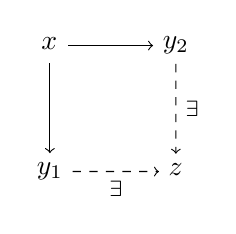
\begin{tikzpicture}[scale=0.8]
        \node (x) at (0,0) {$x_{\vphantom{2}}$};
        \node (y1) at (0,-2) {$y_1$};
        \node (y2) at (2,0) {$y_2$};
        \node (z) at (2,-2) {$z_{\vphantom{1}}$};
        \draw[->] (x) -- (y1);
        \draw[->,dashed] (y1) to node[below] {\footnotesize$\exists$} (z);
        \draw[->] (x) -- (y2);
        \draw[->,dashed] (y2) to node[right] {\footnotesize$\exists$} (z);
    \end{tikzpicture}
    \caption{The diamond property.}
    \label{fig:diamond-property}
\end{marginfigure}

\begin{lemma}
    \label{lem:normal-form-uniqueness}
    If the relation $\to$ on $X$ is Church--Rosser, then any element of $X$ has at most one normal form. If $\to$ is also weakly normalising, then every element has a unique normal form.
\end{lemma}

\begin{proof}
    Let $x \in X$, and let $y_1$ and $y_2$ be normal forms of $x$. Since $\to^*$ has the diamond property there is a $z \in X$ such that $y_1 \to^* z$ and $y^*2 \to^* z$. But since $y_1$ and $y_2$ are irreducible, we must then have $y_1 = z = y_2$. The second claim is obvious.
\end{proof}


\subsection{Reduction in ASTs}\label{sec:reduction-in-ASTs}

Abstract reduction systems are very general. In the context of programming languages (or formal systems such as the $\lambda$-calculus), reductions are induced by the structure of the language in the following way.

Given variables $\setVarAST$ and operators $\setOp$, a \keyword{context}\index[subject]{context} is an AST from $\setAST{\setVarAST}{\setOp}$ in which one sub-AST has been replaced by a \enquote{hole}\index[subject]{hole}, denoted \enquote{$\hole$}\index[notation]{*-aaaahole@$\hole$ (hole)}. More precisely, the set of contexts is defined recursively by the rules
%
\begin{mathparpagebreakable}
    \inferrule{ }{
        \phantom{x}\hole\phantom{x}
    }
    \and
    \inferrule{
        C
    }{
        \phi(\seq{x}_1.a_1 ; \ldots ; \seq{x}_{i-1}.a_{i-1} ; \seq{x}_i.C ; \seq{x}_{i+1}.a_{i+1} ; \ldots ; \seq{x}_n.a_n)
    }
\end{mathparpagebreakable}
%
using the same notation for variables and ASTs as in the definition of $\setAST{\setVarAST}{\setOp}$. If $C$ is a context and $a$ is an AST, then we write $C[a]$\index[notation]{cz-Ca@$C[a]$}\index[notation]{ex-Ee@$E[e]$} for the AST obtained by replacing the hole in $C$ by $a$. We leave it to the reader to provide a recursive definition of the function $C \mapsto C[a]$. Contrary to substitutions which are capture-avoiding, replacement of the hole in a context is supposed to be capturing. Hence we do \emph{not} identify $\alpha$-equivalent contexts, nor the AST replacing the hole therein.

Any context $C$ gives rise to a map $\setAST{\setVarAST}{\setOp} \to \setAST{\setVarAST}{\setOp}$ given by $a \mapsto C[a]$. This in turn induces a composition on contexts such that $C' \circ C$\index[notation]{****-@$\circ$ (composition of contexts)} maps $a$ to $C'[C[a]]$.

Let $\calC$ be a collection of contexts.\blfootnote{In the classical theory of the $\lambda$-calculus we usually only consider the case where $\calC$ is the set of all contexts. In the study of programming languages we will need to consider different classes of contexts, see \cref{sec:evaluation-contexts} and \cref{sec:contextual-equivalence}.} A binary relation $R$ on $\setAST{\setVarAST}{\setOp}$ is \keyword{$\calC$-compatible}\index[subject]{C-compatible@$\calC$-compatible} if $(a,a') \in R$ implies $(C[a],C[a']) \in R$ for all $a,a' \in \setAST{\setVarAST}{\setOp}$ and all $C \in \calC$. The \keyword{$\calC$-compatible closure}\index[subject]{C-compatible closure@$\calC$-compatible closure} of $R$ is the smallest $\calC$-compatible relation extending $R$. The set $\calC$ will usually be clear from context, and in this case we just talk of \enquote{compatibility}.

A \keyword{notion of reduction}\index[subject]{notion of reduction} is simply a binary relation $R$ on $\setAST{\setVarAST}{\setOp}$. This induces various other relations on $\setAST{\setVarAST}{\setOp}$:
%
\begin{itemize}
    \item The compatible closure of $R$ is denoted $\to_R$ and is called the \keyword{one-step $R$-reduction}\index[subject]{reduction!one-step}.
    \item The reflexive and transitive closure of $\to_R$ is denoted $\twoheadrightarrow_R$ and is simply called the \keyword{$R$-reduction}\index[subject]{reduction}.
    \item The equivalence relation generated by $\twoheadrightarrow_R$ is denoted $=_R$ and is called \keyword{$R$-convertibility} or \keyword{$R$-equivalence}\index[subject]{reduction!equivalence}.
\end{itemize}
%
Notice that any of these relations give rise to an abstract reduction system on $\setAST{\setVarAST}{\setOp}$.

In this context, an \keyword{$R$-redex}\index[subject]{reduction!redex} is an AST $a$ such that $(a,b) \in R$ for some AST $b$. In this case $b$ is called an \keyword{$R$-contractum}\index[subject]{reduction!contractum} of $a$. An AST $a$ is called an \keyword{$R$-normal form}\index[subject]{reduction!normal form} if it is irreducible with respect to $\to_R$. If $a \twoheadrightarrow_R b$ where $b$ is an $R$-normal form, then we also say that $b$ is an $R$-normal form \emph{of} $a$. We finally say that a notion of reduction $R$ is Church--Rosser\index[subject]{Church--Rosser} if the one-step $R$-reduction $\to_R$ is.


\section{Partitions and coinduction}

\subsection{Partitions}

Recall that a \keyword{partition}\index[subject]{partition} of a set $X$ is a collection $\calP$ of pairwise disjoint subsets of $X$ such that $X = \bigunion \calP$. Every partition induces an equivalence relation $\sim_{\calP}$ on $X$ such that $x \sim_{\calP} y$ if and only if $x$ and $y$ belong to the same set in $\calP$. Conversely, every equivalence relation $\sim$ on $X$ induces a partition $\calP_\sim$ whose sets are the $\sim$-equivalence classes.

\blfootnote{Note that depending on which kinds of families of sets one is considering, different definitions of fineness or coarseness are appropriate. For instance, one topology is finer than another if the latter is a \emph{subset} of the former.}%
If $\sim$ and $\approx$ are equivalence relations, then we say that $\sim$ is \keyword{finer}\index[subject]{equivalence relation!finer} than $\approx$ (and that $\approx$ is \keyword{coarser}\index[subject]{equivalence relation!coarser} than $\sim$) if $\calP_\sim$ is finer than $\calP_\approx$, i.e., if for every $A \in \calP_\sim$ there is a $B \in \calP_\approx$ with $A \subseteq B$. This equivalent to the property that $x \sim y$ implies $x \approx y$ for all $x,y \in X$. On the other hand, this is equivalent to the inclusion ${\sim} \subseteq {\approx}$, so coarseness and size are synonyms: One equivalence relation is coarser than another if and only if it is larger (as a set).


\subsection{Coinduction}\label{sec:coinduction}

Now notice that \cref{thm:knaster-tarski} (the Knaster--Tarski fixed-point theorem) has the following immediate consequence:

\begin{corollarynoproof}[Principle of coinduction]
    \label{cor:coinduction-abstract}\index[subject]{coinduction}
    Let $L$ be a complete lattice and let $f \colon L \to L$ be monotone. If $y \in P$ is $f$-consistent, then $y \leq \gfp{f}$.
\end{corollarynoproof}
%
In the important special case where $L$ is a power set $\powerset{X}$ and $F \colon \powerset{X} \to \powerset{X}$ is monotone, recall that the principle of induction (cf. \cref{cor:induction-abstract}) allows us to prove that the set $\lfp{F}$ has a certain property $P$, if only we can show that the characteristic set of $P$ is $F$-closed. On the other hand, the above principle of \emph{coinduction} says that to prove that some element $x \in X$ belongs to $\gfp{F}$, it suffices to find an $F$-consistent set containing $x$. 

Returning to relations, while these are not always defined using a generating function, we can sometimes show that some relation of interest $R$ is the largest or coarsest with some property $P$. To show that $xRy$, it thus suffices to find another relation $S$ with property $P$ such that $xSy$. We will take this approach in \cref{chap:logical-relations}.
